\MainChapter{Caracterización del \texorpdfstring{\ac{GRID}}{GRID}}{\topBanner}\label{cap:caracterizacion-grid}
\vspace*{0.7cm}

El Grupo de investigación \ac{GRID} de la Universidad del Quindío desarrolla actividades orientadas a la investigación, formación académica y apropiación de conocimientos relacionados con las tecnologías de la información y las comunicaciones. En este contexto, el grupo dispone de una infraestructura tecnológica que soporta diferentes servicios utilizados para el desarrollo de actividades académicas, investigativas y administrativas, los cuales requieren mecanismos de autenticación y control de acceso para sus usuarios.

Por lo tanto, la caracterización del grupo constituye un elemento de referencia para identificar las necesidades relacionadas con la gestión de identidades y establecer las condiciones técnicas bajo las cuales se desarrolló la propuesta. Asimismo, permite delimitar el alcance de la solución, considerando tanto los servicios que serían integrados como los mecanismos de autenticación y autorización disponibles en cada uno de ellos.

\section{Análisis de stakeholders del \texorpdfstring{\ac{GRID}}{GRID}}

Con el propósito de identificar los actores relacionados con la infraestructura tecnológica del Grupo de Investigación en Redes, Información y Distribución (\ac{GRID}), se llevó a cabo un análisis de stakeholders, cuyos resultados precisaron los diferentes roles, intereses y niveles de influencia que presentan los actores frente a la gestión y utilización de los servicios tecnológicos considerados en el proyecto.

Los principales stakeholders identificados corresponden al Grupo de Investigación \ac{GRID}, los docentes del programa de Ingeniería de Sistemas y Computación y los estudiantes del mismo programa. Estos actores mantienen una relación directa con la infraestructura, aunque con diferentes niveles de participación, influencia e interés.

El Grupo de Investigación \ac{GRID} constituye el principal beneficiario y actor con capacidad de decisión frente al proyecto, debido a que es responsable de la infraestructura tecnológica y de los servicios sobre los cuales se plantea la solución. Su participación resulta fundamental para establecer las necesidades de gestión de usuarios, definir las condiciones de acceso a los recursos y determinar las características que debe cumplir la solución implementada.

Los docentes de Ingeniería de Sistemas y Computación representan usuarios de la infraestructura tecnológica, principalmente en el desarrollo de actividades académicas e investigativas que requieren el acceso a los servicios proporcionados por el \ac{GRID}. Por su relación con estos recursos, presentan interés en disponer de mecanismos que permitan un acceso adecuado a los servicios según las autorizaciones correspondientes.

Por su parte, los estudiantes de Ingeniería de Sistemas y Computación corresponden a usuarios finales de los recursos tecnológicos disponibles. Su participación se relaciona con el uso de los servicios para actividades académicas, prácticas y de formación, por lo que constituyen un grupo directamente afectado por los mecanismos establecidos para gestionar las cuentas y controlar el acceso.

La \autoref{tab:stakeholders} presenta la caracterización de estos stakeholders, considerando su rol, relación con el proyecto, impacto, poder de influencia, interés y compromiso. Esta identificación permite establecer las responsabilidades y expectativas de los principales actores involucrados en el contexto de la solución propuesta.

\begin{table}[H]
	\centering
	\caption{Análisis de stakeholders}
	\label{tab:stakeholders}

	\renewcommand{\arraystretch}{1.25}
	\setlength{\tabcolsep}{4pt}
	\fontsize{7pt}{7pt}\selectfont

	\begin{tabularx}{\textwidth}{|
		>{\raggedright\arraybackslash}p{2.0cm}|
		>{\raggedright\arraybackslash}p{1.7cm}|
		>{\raggedright\arraybackslash}X|
		>{\raggedright\arraybackslash}p{1.5cm}|
		>{\raggedright\arraybackslash}X|
		>{\raggedright\arraybackslash}X|
		>{\raggedright\arraybackslash}p{2.0cm}|}

		\hline
		\textbf{Interesado}                                                                                                                                          &
		\textbf{Rol}                                                                                                                                                 &
		\textbf{Relación}                                                                                                                                            &
		\textbf{Impacto}                                                                                                                                             &
		\textbf{Poder de influencia}                                                                                                                                 &
		\textbf{Interés}                                                                                                                                             &
		\textbf{Compromiso}
		\\
		\hline

		Docentes de Ingeniería de Sistemas                                                                                                                           &
		Usuarios clave                                                                                                                                               &
		Utilizarán los servicios tecnológicos del GRID en actividades académicas e investigativas que requieran acceso a los recursos de la infraestructura          &
		Medio-Alto                                                                                                                                                   &
		Medio, pueden influir en la adopción mediante el uso de los servicios, aunque no tienen responsabilidad directa sobre las decisiones de la infraestructura   &
		Medio-Alto, requieren mecanismos de acceso que faciliten el uso de los servicios tecnológicos de acuerdo con los permisos establecidos                       &
		Medio, condicionado por la utilidad y facilidad de uso de los mecanismos de autenticación y acceso
		\\
		\hline

		Estudiantes de Ingeniería de Sistemas                                                                                                                        &
		Usuarios finales                                                                                                                                             &
		Utilizarán los servicios tecnológicos disponibles para actividades académicas, prácticas y de formación                                                      &
		Bajo-Medio                                                                                                                                                   &
		Bajo, no participan directamente en las decisiones sobre la infraestructura, aunque su experiencia de uso permite valorar el funcionamiento de la solución   &
		Medio, debido a la necesidad de acceder a los recursos tecnológicos requeridos para sus actividades académicas                                               &
		Bajo-Medio, relacionado con la disponibilidad y facilidad de acceso a los servicios
		\\
		\hline

		Grupo de Investigación GRID                                                                                                                                  &
		Beneficiario principal                                                                                                                                       &
		Proporciona y administra la infraestructura tecnológica, define las necesidades de gestión de usuarios y establece las condiciones de acceso a los servicios &
		Alto                                                                                                                                                         &
		Alto, tiene capacidad para definir las condiciones de implementación y tomar decisiones sobre la gestión de la infraestructura                               &
		Alto, busca mejorar la administración de las cuentas de usuario, centralizar la gestión de identidades y facilitar el control de acceso a sus servicios      &
		Alto, debido a su responsabilidad directa sobre la infraestructura y a los beneficios esperados de la solución
		\\
		\hline
	\end{tabularx}
\end{table}


\section{Integrantes y áreas de trabajo del \texorpdfstring{\ac{GRID}}{GRID}}

El Grupo de Investigación en Redes, Información y Distribución (\ac{GRID}) está conformado por docentes e investigadores vinculados a diferentes áreas de conocimiento relacionadas con las tecnologías de la información y las comunicaciones. Sus integrantes participan en actividades de investigación, desarrollo y formación, haciendo uso de los recursos y servicios tecnológicos disponibles en la infraestructura del grupo.

A continuación, se presenta una lista de los integrantes actuales del grupo, junto
con sus respectivas líneas de trabajo y áreas de especialización:

\begin{itemize}
	\item \href{https://scienti.minciencias.gov.co/cvlac/visualizador/generarCurriculoCv.do?cod_rh=0000210897}{\textbf{Christian Andrés Candela Uribe}}: Microservicios, desarrollo de software, minería de datos, infraestructura \ac{TI}.
	\item \href{https://scienti.minciencias.gov.co/cvlac/visualizador/generarCurriculoCv.do?cod_rh=0001383939}{\textbf{Luis Eduardo Sepúlveda Rodríguez}}: Infraestructura \ac{TI}, \ac{HPC}, computación paralela.
	\item \href{https://scienti.minciencias.gov.co/cvlac/visualizador/generarCurriculoCv.do?cod_rh=0001343801}{\textbf{Carlos Eduardo Gómez Montoya}}: Redes, ingeniería de software, cloud computing.
	\item \href{https://scienti.minciencias.gov.co/cvlac/visualizador/generarCurriculoCv.do?cod_rh=0001398775}{\textbf{Sergio Augusto Cardona Torres}}: Big data y análisis de datos, ingeniería de software, sistemas adaptativos, informática educativa.
	\item \href{https://scienti.minciencias.gov.co/cvlac/visualizador/generarCurriculoCv.do?cod_rh=0000193550}{\textbf{Sonia Jaramillo Valbuena}}: Big data, electroquímica, inteligencia artificial.
	\item \href{https://scienti.minciencias.gov.co/cvlac/visualizador/generarCurriculoCv.do?cod_rh=0000283495}{\textbf{Julián Esteban Gutiérrez Posada}}: Microservicios, desarrollo de software, minería de datos, infraestructura \ac{TI}, \ac{HPC}, computación paralela, redes, ingeniería de software.
\end{itemize}

La diversidad de áreas de trabajo de los integrantes del \ac{GRID} aporta capacidades complementarias en infraestructura de \ac{TI}, redes, desarrollo de software y gestión de servicios tecnológicos. Esta combinación de conocimientos favorece la atención de las necesidades técnicas asociadas con la infraestructura del grupo y proporciona las capacidades necesarias para integrar y administrar los diferentes servicios que la conforman. En este contexto, la experiencia de sus integrantes constituye un elemento relevante para la implementación de mecanismos orientados a centralizar la gestión de identidades y facilitar el control de acceso a los recursos tecnológicos disponibles.

\section{Misión del \texorpdfstring{\ac{GRID}}{GRID}}

La misión del \ac{GRID} se encuentra alineada con los propósitos institucionales de la Universidad del Quindío. A continuación, se presenta la misión de la universidad:

\begin{quote}
	\textit{La Universidad del Quindío, como Institución pública de alta calidad, forma ciudadanos para el mundo actual que contribuyen a la transformación social, cultural, tecnológica, económica y ambiental, sustentada en la transferencia como fundamento investigativo y la extensión como eje del desarollo territorial. \citep{uniquindio2026}}
\end{quote}

A partir de esta misión, se identifican los siguientes ejes fundamentales:

\begin{itemize}
	\item \textbf{Docencia:} Orientada a la formación de ciudadanos para el mundo actual, promoviendo el desarrollo de conocimientos y capacidades que les permitan contribuir a la transformación de su entorno.

	\item \textbf{Investigación:} Enfocada en la generación y transferencia de conocimiento como fundamento para contribuir a la transformación social, cultural, tecnológica, económica y ambiental.

	\item \textbf{Extensión y Desarrollo Social:} Dirigida a fortalecer la relación de la Universidad con su entorno y contribuir al desarrollo territorial mediante la transferencia y aplicación del conocimiento generado.

	\item \textbf{Responsabilidad Social:} Orientada a la formación de ciudadanos comprometidos con la transformación de su entorno y con las necesidades sociales, culturales, tecnológicas, económicas y ambientales de la sociedad.
\end{itemize}

\section{Visión del \texorpdfstring{\ac{GRID}}{GRID}}

La misión de la Universidad del Quindío se complementa con su visión institucional, la cual también es adoptada por el \ac{GRID}. A continuación se presenta la visión de la universidad:

\begin{quote}
	\textit{La Universidad del Quindío en el 2040 será una institución líder en procesos de impacto territorial, transformadora, innovadora, adaptable, con articulación y prospectiva glocal, que forme ciudadanos íntegros, comprometidos con la sociedad, con pensamiento crítico, sensibilidad social, y capacidad para afrontar los desafíos cambiantes del mundo. \citep{uniquindio2026}}
\end{quote}

A partir de esta visión, se identifican los siguientes enfoques estratégicos:

\begin{itemize}
	\item \textbf{Gestión:} Orientada hacia una institución líder, adaptable e innovadora, con capacidad para responder a los cambios y desafíos del entorno.

	\item \textbf{Docencia:} Enfocada en la formación de ciudadanos íntegros, con pensamiento crítico, sensibilidad social y capacidades para afrontar los desafíos cambiantes del mundo.

	\item \textbf{Investigación:} Orientada a generar conocimiento y capacidades que contribuyan a procesos de transformación e impacto territorial, articulándose con las necesidades y desafíos del entorno.

	\item \textbf{Extensión y Desarrollo Social:} Dirigida a fortalecer el impacto territorial de la Universidad mediante la articulación con su entorno y la generación de iniciativas que contribuyan a la transformación de la sociedad.

	\item \textbf{Responsabilidad Social:} Orientada a formar ciudadanos comprometidos con la sociedad, con sensibilidad frente a las necesidades de su entorno y capacidad para contribuir a procesos de transformación con impacto territorial.
\end{itemize}

\section{Impacto del proyecto en el \texorpdfstring{\ac{GRID}}{}}

El proyecto contribuye a fortalecer la gestión de la infraestructura tecnológica del \ac{GRID} mediante la centralización de las identidades y el acceso a los servicios, favoreciendo una administración más organizada de las cuentas de usuario y de los permisos asociados a los recursos tecnológicos.

Asimismo, puede mejorar la gestión operativa relacionada con los usuarios al reducir la dispersión de las cuentas entre los diferentes servicios y establecer una base común para su administración, facilitando las actividades de incorporación, modificación y control de los accesos.

En consecuencia, el proyecto proporciona al \ac{GRID} una base tecnológica orientada a una gestión más uniforme de los usuarios y los accesos a los servicios, que puede favorecer la administración de la infraestructura y su evolución conforme surjan nuevas necesidades.

\section{Descripción de la oportunidad}

La centralización de la gestión de identidades y del acceso a los servicios tecnológicos del \ac{GRID} representa una oportunidad para mejorar la administración de las cuentas de usuario y facilitar el control de los accesos a los recursos de la infraestructura. Esta oportunidad surge de la necesidad de contar con mecanismos que permitan gestionar de manera organizada las identidades de los usuarios y su relación con los diferentes servicios tecnológicos utilizados por el grupo.

\section{Entrevista con integrante del grupo \texorpdfstring{\ac{GRID}}{}}

Con el propósito de conocer la situación de la gestión de usuarios y el acceso a los servicios tecnológicos del \ac{GRID}, se entrevistó a un integrante del grupo relacionado con la administración y utilización de su infraestructura tecnológica. Esta actividad aportó información sobre la forma en que se gestionan actualmente las cuentas de usuario, los mecanismos de autenticación y autorización empleados en los servicios, así como las principales necesidades identificadas para mejorar la administración de los recursos tecnológicos.

El instrumento utilizado correspondió a una entrevista semiestructurada, mediante la cual se abordaron aspectos relacionados con la administración de usuarios, el acceso a los servicios, las políticas de seguridad, el control de permisos, la integración entre servicios y las necesidades futuras de la infraestructura. Las respuestas obtenidas fueron analizadas para identificar aquellos aspectos que pudieran ser considerados dentro del alcance del proyecto.

A continuación, en la \autoref{fig:vista-general-entrevista}, se presenta una vista general de la entrevista. La versión completa de esta se encuentra disponible en el apéndice \ref{sec:entrevista}.

\begin{figure}[H]
	\centering
	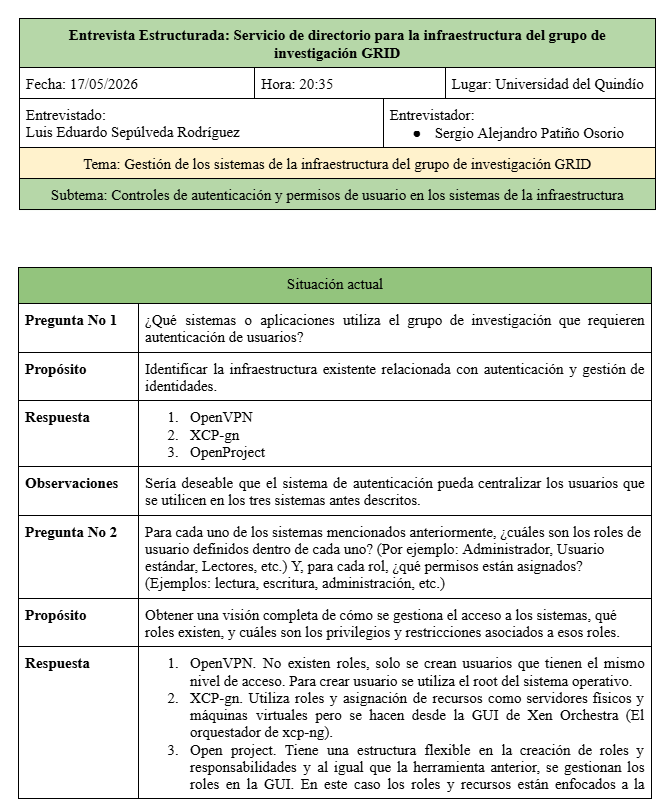
\includegraphics[width=0.7\textwidth]{imagenes/figuras/II-desarrollo-metodologico/cap10-caracterizacion-grid/vista-general-entrevista.png}
	\caption{Vista general de la entrevista}
	\label{fig:vista-general-entrevista}
\end{figure}

\subsection{Resultados de la entrevista}

A partir de la información recopilada se identificó que la gestión de las cuentas de usuario y el acceso a los diferentes servicios tecnológicos constituían aspectos relevantes para la administración de la infraestructura del \ac{GRID}. La existencia de diferentes servicios con mecanismos propios de autenticación implicaba considerar la necesidad de establecer una gestión más centralizada de las identidades y facilitar la administración de las cuentas.

Asimismo, se identificó la necesidad de establecer mecanismos que permitieran administrar el ciclo de vida de las cuentas de usuario, considerando actividades como su creación, modificación y eliminación. De manera complementaria, se evidenció la importancia de establecer políticas relacionadas con la seguridad de las credenciales y de controlar el acceso a los servicios de acuerdo con los permisos asignados a cada usuario.

Otro aspecto identificado correspondió a la necesidad de fortalecer la capacidad de supervisar los accesos realizados a los servicios y disponer de información que pudiera ser utilizada para fines de seguimiento y auditoría. También se consideró relevante que la solución pudiera integrarse con diferentes servicios tecnológicos y mantener la posibilidad de incorporar nuevos recursos conforme evolucionara la infraestructura del grupo.

La entrevista también permitió identificar expectativas relacionadas con el fortalecimiento de los mecanismos de autenticación y con la recuperación o restablecimiento de las credenciales de los usuarios.

\subsection{Identificación de necesidades, problemas y oportunidades}

Los resultados de la entrevista fueron organizados en términos de \ac{NPO}, con el propósito de establecer una relación entre la situación identificada en el \ac{GRID} y los requerimientos que posteriormente orientarían el desarrollo del proyecto.

\begingroup
\fontsize{8pt}{9pt}\selectfont
\renewcommand{\arraystretch}{1.25}
\setlength{\tabcolsep}{3pt}

\begin{longtable}{|
	>{\centering\arraybackslash}p{0.09\dimexpr\textwidth-6\tabcolsep-5\arrayrulewidth\relax}|
	>{\centering\arraybackslash}p{0.12\dimexpr\textwidth-6\tabcolsep-5\arrayrulewidth\relax}|
	>{\raggedright\arraybackslash}p{0.34\dimexpr\textwidth-6\tabcolsep-5\arrayrulewidth\relax}|
	>{\raggedright\arraybackslash}p{0.45\dimexpr\textwidth-6\tabcolsep-5\arrayrulewidth\relax}|}

	\caption{Necesidades, problemas y oportunidades identificados en la entrevista}
	\label{tab:npo}
	\\
	\hline
	\textbf{ID}                                                                                                     &
	\textbf{Tipo}                                                                                                   &
	\textbf{Necesidad, problema u oportunidad}                                                                      &
	\textbf{Situación identificada}
	\\
	\hline
	\endfirsthead

	\hline
	\textbf{ID}                                                                                                     &
	\textbf{Tipo}                                                                                                   &
	\textbf{Necesidad, problema u oportunidad}                                                                      &
	\textbf{Situación identificada}
	\\
	\hline
	\endhead

	NPO-01                                                                                                          &
	Problema                                                                                                        &
	La autenticación de usuarios se encuentra distribuida entre los diferentes sistemas del grupo de investigación. &
	No existe un servicio unificado de autenticación y la gestión de las cuentas se realiza de manera individual en cada herramienta.
	\\
	\hline

	NPO-02                                                                                                          &
	Necesidad                                                                                                       &
	Centralizar las cuentas de usuario de OpenVPN, Xen Orchestra y OpenProject.                                     &
	Se identificó la necesidad de centralizar las cuentas utilizadas en los diferentes sistemas.
	\\
	\hline

	NPO-03                                                                                                          &
	Problema                                                                                                        &
	La creación, verificación y cierre de cuentas se realiza manualmente.                                           &
	Las actividades relacionadas con la administración de las cuentas se ejecutan de forma manual, situación considerada crítica debido a la necesidad de relacionar la vigencia de las cuentas con situaciones como la terminación de trabajos de grado.
	\\
	\hline

	NPO-04                                                                                                          &
	Necesidad                                                                                                       &
	Automatizar el ciclo de vida de las cuentas de usuario.                                                         &
	Se requiere automatizar actividades como la provisión, desprovisión, registro, verificación, revocación y expiración de las credenciales.
	\\
	\hline

	NPO-05                                                                                                          &
	Problema                                                                                                        &
	No existe una política estandarizada de contraseñas y acceso.                                                   &
	Se utilizan prácticas no estandarizadas y dependientes de cada usuario para la gestión de contraseñas y acceso.
	\\
	\hline

	NPO-06                                                                                                          &
	Necesidad                                                                                                       &
	Establecer políticas coherentes de creación de usuarios y contraseñas.                                          &
	Se requiere establecer un patrón coherente y repetible para la gestión de usuarios y credenciales, considerando buenas prácticas y estándares.
	\\
	\hline

	NPO-07                                                                                                          &
	Problema                                                                                                        &
	No se realizan revisiones periódicas de los accesos.                                                            &
	No existen mecanismos establecidos para realizar revisiones periódicas de los accesos de los usuarios.
	\\
	\hline

	NPO-08                                                                                                          &
	Necesidad                                                                                                       &
	Implementar mecanismos de control y monitoreo de los accesos.                                                   &
	Se requiere contar con mecanismos para controlar y monitorear los accesos, preferiblemente con capacidad de supervisión en tiempo real.
	\\
	\hline

	NPO-09                                                                                                          &
	Problema                                                                                                        &
	No existe un registro centralizado de las actividades relacionadas con usuarios y administradores.              &
	Las actividades asociadas con la gestión de usuarios y administradores no se registran actualmente de manera centralizada.
	\\
	\hline

	NPO-10                                                                                                          &
	Necesidad                                                                                                       &
	Contar con trazabilidad y auditoría de las actividades de gestión de accesos.                                   &
	Se requiere registrar las actividades relacionadas con la gestión de accesos para facilitar su seguimiento y posterior auditoría.
	\\
	\hline

	NPO-11                                                                                                          &
	Necesidad                                                                                                       &
	Mantener una autorización diferenciada para cada sistema aun cuando las cuentas estén centralizadas.            &
	Se requiere que la centralización de las cuentas no implique que todos los usuarios tengan acceso a los mismos sistemas.
	\\
	\hline

	NPO-12                                                                                                          &
	Necesidad                                                                                                       &
	Fortalecer los mecanismos de autenticación mediante políticas de contraseñas, MFA, certificados y tokens.       &
	Durante la entrevista se consideró necesario fortalecer la autenticación mediante estos mecanismos, de acuerdo con las necesidades de los servicios.
	\\
	\hline

	NPO-13                                                                                                          &
	Necesidad                                                                                                       &
	Establecer mecanismos seguros para la recuperación de contraseñas.                                              &
	Se planteó la posibilidad de utilizar mecanismos de recuperación automática mediante correo electrónico o un segundo factor.
	\\
	\hline

	NPO-14                                                                                                          &
	Oportunidad                                                                                                     &
	Preparar la infraestructura de autenticación para incorporar activos de información de mayor valor.             &
	Aunque el impacto actual de un acceso no autorizado se considera medio, se prevé la incorporación futura de activos de mayor valor.
	\\
	\hline
\end{longtable}
\endgroup


La identificación de estos aspectos permitió establecer una base para la definición de los requerimientos funcionales y no funcionales considerados en el proyecto. De esta manera, los hallazgos obtenidos durante la entrevista fueron utilizados como insumo para orientar la identificación de una tecnología de servicio de directorio y posteriormente evaluar su capacidad para responder a las necesidades planteadas en el contexto del \ac{GRID}.
